%%%%%%%%%%%%%%%%%%%%%%%%%%%%%%%%%%%%%%%%%%%%%%%%%%%
%% LaTeX book template                           %%
%% Author:  Amber Jain (http://amberj.devio.us/) %%
%% License: ISC license                          %%
%%%%%%%%%%%%%%%%%%%%%%%%%%%%%%%%%%%%%%%%%%%%%%%%%%%

\documentclass[a4paper,11pt,oneside]{book}

% pacotes utilizados
\usepackage[T1]{fontenc}
\usepackage[utf8]{inputenc}
\usepackage{lmodern}
\usepackage{hyperref}
\usepackage{graphicx}
\usepackage[portuguese]{babel}
\usepackage{amsfonts}
\usepackage[usenames,dvipsnames]{xcolor}
\usepackage{mathtools}
\usepackage{amssymb} % alguns simbolos matematicos
\usepackage{mathrsfs} % letras cursivas
\usepackage{listings} % coding examples in latex file
\usepackage{xcolor} % changing colors
\usepackage{amsthm} % definir estilo do teorema
\usepackage[hang,flushmargin]{footmisc} % remove footnote's identation
\usepackage{cancel} % para poder colocar o tracinho de cancelamento
\usepackage{tikz} % to draw Venn's diagrams
\usepackage{amsmath} % to write a function by cases
\usepackage{graphicx} % to set a images directory

\graphicspath{{./images/}}

% dark theme no pdf
\pagecolor[rgb]{0.1,0.1,0.1} %black
\color[rgb]{0.9,0.9,0.9} %grey

% criando o modelo de definicoes/teoremas/fatos/demonstracoes
\theoremstyle{definition}

\newtheoremstyle{break}% name
  {10pt}%         Space above, empty = `usual value'
  {10pt}%         Space below
  {}% Body font
  {}%         Indent amount (empty = no indent, \parindent = para indent)
  {\bfseries}% Thm head font
  {}%        Punctuation after thm head
  {\newline}% Space after thm head: \newline = linebreak
  {}%         Thm head spec

\theoremstyle{break}

% definindo as categorias de formalidade
\newtheorem{definition}{Definição}[section]
\newtheorem{fact}{Fato}[section]
\newtheorem{demonstration}{Demonstração}[section]
\newtheorem{theorem}{Teorema}

% tirando identação dos paragrafos
\setlength{\parindent}{0ex}

% setting das cores quando usar codigo python
\definecolor{codegreen}{rgb}{0,0.6,0}
\definecolor{codegray}{rgb}{0.5,0.5,0.5}
\definecolor{codepurple}{rgb}{0.58,0,0.82}
\definecolor{backcolour}{rgb}{0.95,0.95,0.92}

\lstdefinestyle{mystyle}{
    backgroundcolor=\color{backcolour},   
    commentstyle=\color{codegreen},
    keywordstyle=\color{magenta},
    numberstyle=\tiny\color{codegray},
    stringstyle=\color{codepurple},
    basicstyle=\ttfamily\footnotesize,
    breakatwhitespace=false,         
    breaklines=true,                 
    captionpos=b,                    
    keepspaces=true,                 
    numbers=left,                    
    numbersep=5pt,                  
    showspaces=false,                
    showstringspaces=false,
    showtabs=false,                  
    tabsize=2
}

\lstset{style=mystyle}

% dedicatoria 
% Source: http://www.tug.org/pipermail/texhax/2010-June/
\newenvironment{dedication}
{
   \cleardoublepage
   \thispagestyle{empty}
   \vspace*{\stretch{1}}
   \hfill\begin{minipage}[t]{0.66\textwidth}
   \raggedright
}
{
   \end{minipage}
   \vspace*{\stretch{3}}
   \clearpage
}

% Chapter quote at the start of chapter        %
% Source: http://tex.stackexchange.com/a/53380 %
\makeatletter
\renewcommand{\@chapapp}{}% Not necessary...
\newenvironment{chapquote}[2][2em]
  {\setlength{\@tempdima}{#1}%
   \def\chapquote@author{#2}%
   \parshape 1 \@tempdima \dimexpr\textwidth-2\@tempdima\relax%
   \itshape}
  {\par\normalfont\hfill--\ \chapquote@author\hspace*{\@tempdima}\par\bigskip}
\makeatother


%%%%%%%%%%%%%%%%%%%%%%%%%%%%%%%%%%%%%%%%%%%%%%%%%%%
% First page of book which contains 'stuff' like: %
%  - Book title, subtitle                         %
%  - Book author name                             %
%%%%%%%%%%%%%%%%%%%%%%%%%%%%%%%%%%%%%%%%%%%%%%%%%%%
% Book's title and subtitle
\title{\Huge \textbf{Microeconomia} \\ 
\Large Tradução da 9 edição \\
\huge Hal R. Varian}

% Author
\author{
\textsc{Resumo e Adaptação por:} \\
\textsc{Bruno de M. Ruas}
}

\begin{document}

\frontmatter
\maketitle

\tableofcontents
%\listoffigures
%\listoftables

\mainmatter

%%%%%%%%%%%%%%%%%%%%%%%% PART %%%%%%%%%%%%%%%%%%%%%%%%
\part{Preparativos}

%%%%%%%%%%%%%%%%%%%%%%%% CHAPTER %%%%%%%%%%%%%%%%%%%%%%%%
\chapter{Matemática}

\begin{chapquote}{página 1.008}
	``Revisão breve de alguns conceitos matemáticos utilizados no texto''.
\end{chapquote}

Bem vindo ao meu resumo do livro do prof. Varian. Ao contrário do que ele fez, eu preferi trazer o apêndice de matemática pro começo do material porque aqui nós vamos ver as ferramentas que serão usadas para a explicação dos conceitos teóricos ao longo do material.
\\
\\
Aqui a gente só vai dar um overview básico nos conceitos. Não tenha dúvida que alguém mais experimentado em matemática torceria o nariz pra algumas definições dadas aqui. Mas o objetivo é te dar um "norte"\ a respeito de alguns conceitos normalmente usados. Não se assuste com a simplicidade de algumas coisas. Melhor garantir agora do que sofrer mais pra frente no texto.

\section{Funções}

Sejam dois números quaisquer $x$ e $y$, uma \textbf{função} ou \textbf{transformação} é uma regra que descreve uma relação entre eles.
\\
\\
Para demonstrar que existe alguma dependência entre duas variáveis usamos a notação $y = f(x)$, onde nossa variável $y$ (chamada de \textbf{dependente}) é o resultado de alguma transformação (denotada pelo símbolo $"f"$) realizada em $x$ (nossa variável \textbf{independente}).
\\
\\
Não é raro ter uma variável dependente relacionada a várias outras variáveis. Nesses casos é comum o uso da notação anterior com a adição das novas incógnitas. Algo como $y = f(x_1,x_2,...,x_n)$.

\section{Gráficos}

Não tem muito o que falar aqui. Dá uma lida lá na página 1010.

\section{Propriedades de funções}

Uma função pode ter algumas características que facilitam a sua descrição. Aqui temos algumas que serão usadas ao longo do curso:
\\
\\
Uma \textbf{função contínua} é aquela que não possui nenhum "salto"\ ou "quebra". 
\\
\\
Uma \textbf{função suave} é aquela que não tem "dobras"\ nem "cantos".
\\
\\
Uma \textbf{função monotônica} é aquela que sempre segue o mesmo sentido (ou crescendo ou decrescendo) sem nunca mudar de sentido. 
Quando é crescente a medida que $x$ cresce, chamaremos de \textbf{função monotônica crescente}. Quando descrescer a medida que $x$ crescer, chamaremos de \textbf{função monotônica decrescente}.

\section{Funções inversas}

Uma das implicações de quando uma função é monotônica é que, para cada $x$, sempre existirá apenas um único $y$ associado. 
\\
\\
Uma \textbf{função inversa} é a função que, sempre que colocarmos um $y$ como variável independente teremos como resultado um $x$ de alguma função anterior.\footnote{Eu tentei não deixar confuso mas se ficou com dúvida, pesquisa um pouco sobre o tema.}

\section{Equações e identidades}

Podemos relacionar dois ou mais elementos por meio do uso de \textbf{equações} (usando o símbolo da igualdade "$=$"). Onde as suas respectivas \textbf{soluções} são os valores atribuíveis as incógnitas que assegurem a validade da relação proposta.
\\
\\
Uma \textbf{identidade} (que tem o símbolo dado por "$\equiv$") é um tipo de relação onde sempre haverá as soluções independentemente de quais valores suas variáveis assumam.

\section{Funções lineares}

Chamamos de \textbf{função linear}, qualquer função da forma $y = ax + b$. Fique atento porque uma função linear pode ser expressa de maneira implícita (ou seja, será necessário desenvolver um pouco a álgebra até que se chegue numa equação no formato da definição).

\section{Variações e taxas de variação}

Usamos o símbolo "$\Delta$"\footnote{O nome é "delta".} para denotar a variação de alguma variável. Ou seja, se tivemos uma variável qualquer $x$ que teve seu valor alterado de $x^1$ para $x^2$, então:

$$ \Delta x = x^2 - x^1 $$
ou também
$$ x^2 = x^1 + \Delta x $$
\\
Normalmente, usamos o delta quando falamos de \textbf{pequenas variações} ou, como os economistas falam, \textbf{variações marginais}.
\\
\\
A \textbf{taxa de variação} é obtida pela razão (ou seja, pela divisão) de duas variações. Seja a função $y = f(x)$, sempre que tivemos um $\Delta x > 0$ também teremos algum $\Delta y \neq 0$. A taxa de variação de $y$ em relação à $x$ é dada por:

$$ \frac{\Delta y}{\Delta x} = \frac{y^2 - y^1}{x^2 - x^1} = \frac{f(x^1 + \Delta x) - f(x^1)}{\Delta x} $$
\\
É uma medida do quanto $y$ varia a medida que $x$ varia.
\\
\\
Quando uma função é linear, teremos que essa taxa de variação será sempre constante para quaisquer valores de $x$. Como $y = ax + b$, então
\\
\\
\Large $ \frac{\Delta y}{\Delta x} = $ \normalsize
$$ \frac{a+b(x^1 + \Delta x) - (a + bx^1)}{\Delta x} = $$
$$ \frac{\cancel{a}+b(x^1 + \Delta x) \cancel{-a} - bx^1)}{\Delta x} = $$
$$ \frac{\cancel{bx^1} + b \Delta x \cancel{- bx^1}}{\Delta x} = $$
$$ \frac{b \cancel{\Delta x}}{\cancel{\Delta x}} = b  $$

Para as funções não lineares, essa propriedade não é observada. Tomemos $y = f(x) = x^2$ como exemplo,
\\
\\
\Large $ \frac{\Delta y}{\Delta x} = $ \normalsize
$$ \frac{(x + \Delta x)^2 - x^2}{\Delta x} = $$ 
$$  \frac{\cancel{x^2} + 2x \Delta x + (\Delta x)^2 \cancel{-x^2}}{\Delta x} = $$
$$  \frac{2x \cancel{\Delta x} + \Delta x . \cancel{\Delta x}}{\cancel{\Delta x}} = $$
$$  2x + \Delta x $$
\\
Ou seja, entra no resultado da taxa de variação o valor de $x$ e a magnitude da variação, dada por $\Delta x$.

\section{Inclinações e interceptos}

Já aprendemos como calcular a taxa de variação de uma função. Graficamente falando, essa é a medida da inclinação da curva da função entre os dois pontos que formam o delta da variável independente. 
\\
\\
Em uma função linear, a inclinação da curva sempre será a mesma independente da magnitude da variação. No caso das funções não lineares, a inclinação é dada pela \textbf{reta tangente} ao ponto da curva\footnote{Mais pra frente a gente volta nessa ideia.}.
\\
\\
No caso de uma função linear, $ y = ax + b$, temos alguns pontos que recebem nomes de \textbf{intercepto}. O \textbf{intercepto vertical} ($y^*$) é dado pelo ponto $y = a.0 + b = b$, ou seja, onde $x = 0$. Já o \textbf{intercepto horizontal} ($x^*$) é dado pelo ponto onde $y = ax + b = 0 $, ou seja, $ x = \frac{-b}{a}$.

\section{Valores absolutos e logaritmos}

O \textbf{valor absoluto} de um número $x$ qualquer é definido pela função $f(x)$ do seguinte modo:

\[ f(x) = |x| = \begin{cases} x & se \ x \geqslant \\ -x & se \ x < 0 \end{cases} \]
\\
\\
Você já deve ter visto no ensino médio que o \textbf{logaritmo natural} ou \textbf{log} de um número é uma função escrita como $y = lnx$ ou $y = ln(x)$ e que possui as seguintes propriedades:

\begin{itemize}
 \item Se $x,y > 0$, então, $ ln(xy) = ln(x) + ln(y) $
 \item $ ln(e) = 1 $
 \item $ ln(x^y) = y ln(x) $
\end{itemize}

\section{Derivadas}

Você deve lembrar desse conceito das aulas de matemática no primeiro período. A \textbf{derivada} da função $f(x)$ será dada por:

$$ f'(x) = \frac{df(x)}{dx} = \lim_{\Delta x \to 0} \frac{f(x + \Delta x) - f(x)}{\Delta x} $$
\\
Mas perai, a gente acabou de ver um conceito muito parecido no ponto 1.7. E é isso mesmo, a derivada é o cálculo da taxa de variação à medida que aplicamos o limite\footnote{Vá pesquisar se você não souber o que é isso.} até $0$ para nosso $\Delta x$.
\\
\\
\textbf{Comentário}: Essa técnica é muito importante ao longo de quase todos os tópicos desse curso. Volte nas apostilas e nas listas de derivadas caso seja necessário.

\section{Derivadas segundas}

Já vimos que a deriva nos permite saber a inclinação da reta tangente da nossa função genérica $f(x)$ num determinado ponto. Chamamos de \textbf{derivada segunda} de $f(x)$ a derivada da derivada dessa função.

$$ f''(x) = \frac{d^2f(x)}{dx^2} $$
\\
Nós aplicamos a derivada segunda para descobrirmos a curvatura da função no ponto $x$. Se for positiva, a função é convexa no ponto. Se for negativa, a função é côncava no ponto. Por fim, se for igual a zero, a função será plana.

\section{A regra do produto e da cadeia}

Dadas duas funções $g(x)$ e $h(x)$ Se definirmos uma nova função $f(x) = g(x) h(x)$. A derivada dessa última função é dada pela aplicação da \textbf{regra do produto}:
\\
$$ \frac{df(x)}{dx} = g(x)\frac{dh(x)}{dx} + h(x)\frac{dg(x)}{dx}$$
\\
\\
\textbf{Comentário}: Normalmente a gente vê a regra do produto e da divisão junto. Mas o prof. Varian não colocou essa segunda regra como necessária. Então se eu ver que ficou faltando, eu atualizo esse material.
\\
\\
Agora imagine a situação onde temos uma função dentro de outra função. Dadas as funções $y = g(x)$ e $z = h(y)$, a \textbf{função composta} é dada por $f(x) = h(g(x))$, cuja derivada é obtida pela seguinte regra:

$$ \frac{df(x)}{dx} = \frac{dh(y)}{dy}\frac{dg(x)}{x}$$

\section{Derivadas parciais}

Nós já vimos no ponto 1.1 que funções podem conter mais de uma variável independente. Supondo uma função composta $f(x_1,x_2)$ a sua \textbf{derivada parcial} em relação a $x_1$ será dada por:

$$ \frac{\partial f(x_1,x_2)}{\partial x_1} = 
\lim_{\Delta x_1 \to 0} \frac{f(x_1+\Delta x_1,x_2) - f(x_1,x_2)}{\Delta x_1} $$
\\
similarmente, a derivada parcial em relação a $x_2$ será dada por
\\
$$ \frac{\partial f(x_1,x_2)}{\partial x_2} = 
\lim_{\Delta x_2 \to 0} \frac{f(x_1,x_2+\Delta x_2) - f(x_1,x_2)}{\Delta x_2} $$
\\
A ideia por trás de uma derivada parcial é verificar a taxa de variação entre a nossa função composta em relação a alguma variação de apenas uma das variáveis independentes, ou seja, é como se tratássemos as outras variáveis como constantes.
\\
\\
As propriedades das derivadas parciais são parecidas com as normais. Exceção é a regra da cadeia. Seja a função composta $g(t) = f(x_1(t),x_2(t))$, então a derivada de $g(t)$ em relação a $t$ é dada por:

$$ \frac{dg(t)}{dt} = 
\frac{\partial f(x_1,x_2)}{\partial x_1}\frac{dx_1(t)}{dt} + 
\frac{\partial f(x_1,x_2)}{\partial x_2}\frac{dx_2(t)}{dt} $$
\\
Atente para o fato que as variáveis independentes da nossa função $g(t)$ são as funções $x_1(t)$ e $x_2(t)$ que também têm como variável independente $t$.

\section{Otimização}

A maioria dos modelos utilizados pela Economia podem ser expressos como um problemas de otimização. Matematicamente falando, dada uma função $y = f(x)$ seu valor \textbf{máximo} será dado ponto $x^*$ se $f(x^*) \geqslant f(x)$ para qualquer valor de $x$. Não faz parte do escopo desse apêndice demonstrar isso, então tenha fé que, se uma função for suave, o seu valor máximo é obtido no ponto onde teremos

$$ \frac{df(x^*)}{dx} = 0 $$

e também

$$ \frac{d^2f(x^*)}{dx^2} \leq 0$$
\\
Ou seja, o máximo será o ponto onde a derivada for igual a zero e a derivada segunda for menor igual a zero. Chamamos a primeira de \textbf{condição de primeira ordem} e a segunda de \textbf{condição de segunda ordem}.
\\
\\
Também é muito comum buscarmos a minimização de determinadas funções. Nesse caso, só teremos uma pequena mudança na condição de segunda ordem;

$$ \frac{df(x^*)}{dx} = 0 $$

e também

$$ \frac{d^2f(x^*)}{dx^2} \geq 0$$
\\
No casos das funções compostas suaves, as condições de primeira ordem para os pontos de máximo e mínimo são alcançadas no ponto $(x_{1}^*,x_{2}^*)$ cujas derivadas serão

$$ \frac{\partial f(x_{1}^*,x_{2}^*)}{\partial x_1} = 0 $$
e
$$ \frac{\partial f(x_{1}^*,x_{2}^*)}{\partial x_2} = 0 $$
\\
As condições de segunda ordem são muito mais complexas então não fazem parte do escopo desse curso.

\section{Otimização com restrição}

Saber maximizar ou minimizar uma função é só uma parte do problema de otimização. Na vida real, a esmagadora maioria das situações de otimização está contida dentro de algum limite de possibilidades. A \textbf{otimização com restrição} é a técnica usada para encontrar o ponto de máximo ou mínimo de alguma função dentro de um determinado domínio de possibilidades.

\begin{center}
\LARGE $\stackrel{máx}{\text{\small $x_1,x_2$}} \ \ \stackrel{f(x_1,x_2)}{\ }$ \\
\normalsize $\textrm{de modo que } g(x_1,x_2) = c$
\end{center}

A função $f(x_1,x_2)$ é chamada de \textbf{função objeto} e a equação $g(x_1,x_2) = c$ é chamada de \textbf{restrição}.

%%%%%%%%%%%%%%%%%%%%%%%% CHAPTER %%%%%%%%%%%%%%%%%%%%%%%%
\chapter{Programação}

Caro aluno, com o avanço do poder computacional e da disponibilidade de dados, os economistas não ficaram de fora da revolução tecnológica. Além de todo o arcabouço teórico, matemático, estatístico, histórico e social que você está adquirindo na sua formação, a programação se tornou uma ferramenta indispensável para o processo de análise moderna e merece ser objeto do seu estudo\footnote{Pode até ser que você não tenha alguma matéria de programação na sua grade curricular, mas não se engane, mesmo que seu curso não esteja cobrando, vá estudar por conta própria.}.
\\
\\
Ao longo do livro eu vou construir alguns programas em Python para simular os modelos que a gente for construindo. Não faz parte do escopo desse livro ensinar como fazer isso. Contudo, cada código será disponibilizado em dois links. O primeiro é referente ao repositório no github e o segundo é referente a um notebook no google colab onde você pode executar o modelo sem precisar instalar nada no seu computador.

\section{Capítulo 25 - Monopólio}

\subsection{Demanda Linear e Monopólio (25.2)}

\begin{center}
\href{https://github.com/brunoruas2/Meus_Estudos/blob/main/Microeconomia/Microeconomics\%20-\%20Hal\%20Varian/models/cap25.2-demanda_linear_e_monopolio.py}{
\includegraphics[scale=0.03]{_github_logo.png} \ Código no Github \ 
\includegraphics[scale=0.03]{_github_logo.png}}
\\
\ 
\\
\href{https://colab.research.google.com/drive/1OUK3Z--dv7WMufCLmJ9qDWII1yoVlWVX?usp=sharing}{
\includegraphics[scale=0.08]{_colab_logo.png} Simulação no Google Colab 
\includegraphics[scale=0.08]{_colab_logo.png}}
\end{center}

\subsection{Demanda Elasticidade Constante e Monopólio (25.3)}
\begin{center}
\href{https://github.com/brunoruas2/Meus_Estudos/blob/main/Microeconomia/Microeconomics\%20-\%20Hal\%20Varian/models/cap25.3-demanda_ces_e_monopolio.py}{
\includegraphics[scale=0.03]{_github_logo.png} \ Código no Github 
\includegraphics[scale=0.03]{_github_logo.png}}
\\
\ 
\\
\href{https://colab.research.google.com/drive/1MRJb9DZ7n_Hz2Kp9ng8K7pOcb1DTy_u5?usp=sharing}{
\includegraphics[scale=0.08]{_colab_logo.png} Simulação no Google Colab 
\includegraphics[scale=0.08]{_colab_logo.png}}
\end{center}

%%%%%%%%%%%%%%%%%%%%%%%% PART %%%%%%%%%%%%%%%%%%%%%%%%
\part{Teoria da Escolha}

%%%%%%%%%%%%%%%%%%%%%%%% CHAPTER %%%%%%%%%%%%%%%%%%%%%%%%
\chapter{O Mercado}

\begin{chapquote}{página 3}
	``The theory of sets is a language that is perfectly suited to describing and explaning all types of mathematical structures.''
\end{chapquote}


%\section{A elaboração de um modelo}
%\section{Otimização e equilíbrio}
%\section{A curva de demanda}
%\section{A curva de oferta}
%\section{O equilíbrio de mercado}
%\section{A estática comparativa}
%\section{Outras formas de alocar apartamentos}
%\section{Qual o melhor arranjo?}
%\section{A eficiência de Pareto}
%\section{Comparação entra as formas de alocação de apartamentos}
%\section{Equilíbrio no longo prazo}

%%%%%%%%%%%%%%%%%%%%%%%% CHAPTER %%%%%%%%%%%%%%%%%%%%%%%%
\chapter{Restrição Orçamentária}

%%%%%%%%%%%%%%%%%%%%%%%% CHAPTER %%%%%%%%%%%%%%%%%%%%%%%%
\chapter{Preferências}

%%%%%%%%%%%%%%%%%%%%%%%% CHAPTER %%%%%%%%%%%%%%%%%%%%%%%%
\chapter{Utilidade}

%%%%%%%%%%%%%%%%%%%%%%%% CHAPTER %%%%%%%%%%%%%%%%%%%%%%%%
\chapter{Escolha}

%%%%%%%%%%%%%%%%%%%%%%%% CHAPTER %%%%%%%%%%%%%%%%%%%%%%%%
\chapter{Demanda}

%%%%%%%%%%%%%%%%%%%%%%%% CHAPTER %%%%%%%%%%%%%%%%%%%%%%%%
\chapter{Preferência Revelada}

%%%%%%%%%%%%%%%%%%%%%%%% CHAPTER %%%%%%%%%%%%%%%%%%%%%%%%
\chapter{A Equação de Slutsky}

%%%%%%%%%%%%%%%%%%%%%%%% CHAPTER %%%%%%%%%%%%%%%%%%%%%%%%
\chapter{Restrição Orçamentária}

%%%%%%%%%%%%%%%%%%%%%%%% CHAPTER %%%%%%%%%%%%%%%%%%%%%%%%
\chapter{Comprando e Vendendo}

%%%%%%%%%%%%%%%%%%%%%%%% CHAPTER %%%%%%%%%%%%%%%%%%%%%%%%
\chapter{Escolha Intertermporal}

%%%%%%%%%%%%%%%%%%%%%%%% CHAPTER %%%%%%%%%%%%%%%%%%%%%%%%
\chapter{Mercado de Ativos}

%%%%%%%%%%%%%%%%%%%%%%%% CHAPTER %%%%%%%%%%%%%%%%%%%%%%%%
\chapter{Incerteza}

%%%%%%%%%%%%%%%%%%%%%%%% CHAPTER %%%%%%%%%%%%%%%%%%%%%%%%
\chapter{Ativos de Risco}

%%%%%%%%%%%%%%%%%%%%%%%% CHAPTER %%%%%%%%%%%%%%%%%%%%%%%%
\chapter{O Excedente do Consumidor}

%%%%%%%%%%%%%%%%%%%%%%%% CHAPTER %%%%%%%%%%%%%%%%%%%%%%%%
\chapter{Demanda de Mercado}

%%%%%%%%%%%%%%%%%%%%%%%% PART %%%%%%%%%%%%%%%%%%%%%%%%
\part{Equilíbrio, Econometria e Leilões}

%%%%%%%%%%%%%%%%%%%%%%%% CHAPTER %%%%%%%%%%%%%%%%%%%%%%%%
\chapter{Equilíbrio}

%%%%%%%%%%%%%%%%%%%%%%%% CHAPTER %%%%%%%%%%%%%%%%%%%%%%%%
\chapter{Medição}

%%%%%%%%%%%%%%%%%%%%%%%% CHAPTER %%%%%%%%%%%%%%%%%%%%%%%%
\chapter{Leilões}

%%%%%%%%%%%%%%%%%%%%%%%% CHAPTER %%%%%%%%%%%%%%%%%%%%%%%%
\chapter{Equilíbrio}

%%%%%%%%%%%%%%%%%%%%%%%% PART %%%%%%%%%%%%%%%%%%%%%%%%
\part{Teoria da Firma}

%%%%%%%%%%%%%%%%%%%%%%%% CHAPTER %%%%%%%%%%%%%%%%%%%%%%%%
\chapter{Tecnologia}

%%%%%%%%%%%%%%%%%%%%%%%% CHAPTER %%%%%%%%%%%%%%%%%%%%%%%%
\chapter{Maximização do Lucro}

%%%%%%%%%%%%%%%%%%%%%%%% CHAPTER %%%%%%%%%%%%%%%%%%%%%%%%
\chapter{Minimização de Custos}

%%%%%%%%%%%%%%%%%%%%%%%% CHAPTER %%%%%%%%%%%%%%%%%%%%%%%%
\chapter{Curva de Custo}

%%%%%%%%%%%%%%%%%%%%%%%% CHAPTER %%%%%%%%%%%%%%%%%%%%%%%%
\chapter{Oferta da Empresa}

%%%%%%%%%%%%%%%%%%%%%%%% CHAPTER %%%%%%%%%%%%%%%%%%%%%%%%
\chapter{Oferta da Indústria}

%%%%%%%%%%%%%%%%%%%%%%%% PART %%%%%%%%%%%%%%%%%%%%%%%%
\part{Mercados}

%%%%%%%%%%%%%%%%%%%%%%%% CHAPTER %%%%%%%%%%%%%%%%%%%%%%%%
\chapter{Monopólio}

Anteriormente, fora demonstrado como a oferta pode ser construída da firma individual até a indústria competitiva. Nesse cenário, todos os ofertantes não possuem poder de interferir no preço e na quantidade de equilíbrio do mercado. Mas podemos pensar num caso muito diferente: Como seria o caso onde só exista uma empresa controlando toda a oferta?
\\
\\
Diferente dos casos anteriores, agora nós buscamos construir um modelo de tomada de decisão que leve em consideração a capacidade do monopolista de intervir diretamente no preço de modo a maximizar seus lucros totais.
\\
\\
Existem duas maneiras de enxergar esse problema. Podemos modelar como se o monopolista controlasse o preço e a demanda é quem definiria a quantidade. Ou, ao contrário, podemos modelar como se o monopolista definisse a quantidade a ser produzida e a demanda definiria o seu preço de equilíbrio para essa quantidade.
\\
\\
Independente do modelo, podemos ver que as abordagens são equivalentes. Por facilidade analítica vamos seguir a abordagem de definição da quantidade produzida.

\section{Maximização dos Lucros}

Como vimos nos capítulo 01, estamos diante de um problema de maximização. Sendo mais preciso, nós queremos maximizar o lucro do monopolista dado por $yp(y) - c(y)$ onde $p(y)$ é a demanda inversa\footnote{Lá do capítulo 15. É a função que indica qual deve ser o preço do bem para que seja demanda uma determinada quantidade.} para o mercado, $r(y) = yp(y)$ é a receita do monopolista e $c(y)$ é o custo de produção das $y$ unidades. Podemos resumir nosso problema como

\begin{center}
\LARGE $\stackrel{máx}{\text{\small $y$}} \ \ \stackrel{r(y) - c(y)}{\ }$ \\
\end{center}

A condição de otimização é evidente: A receita marginal deve ser igual ao custo marginal. Se a receita marginal for maior, bastaria aumentar a produção para aumentar os lucros. Se fosse menor, seria necessário reduzir a quantidade produzida afim de elevar o preço a um nível satisfatório. Algebricamente, temos que

$$ \textrm{RM = CMa} $$
$$ ou $$
$$ \frac{\Delta r}{\Delta y} = \frac{\Delta c}{\Delta y} $$
\\
Até aqui a gente tá bem perto da modelagem para as firmas competidoras. O custo marginal é definido pela tecnologia de produção. A mudança acontecerá na receita marginal. 
\\
\\
Como o monopolista tem o poder de intervir no mercado, sempre que ele decidir alterar a produção em $\Delta y$ unidades, haverá dois efeitos na receita. Em primeiro lugar, ele terá um aumento na receita em $p\Delta y$ unidades. Em segundo lugar, como o mercado terá mais bens a sua disposição, ele estará disposto a pagar um preço menor pelas novas unidades, ou seja, $y\Delta p$. O resultado líquido desse efeito é obtido por

$$\Delta r = p \Delta y + y \Delta p$$

$$ \frac{\Delta r}{\Delta y} = 
\frac{p \Delta y}{\Delta y} + 
\frac{y \Delta p}{\Delta y} $$

$$ \phantom{\frac{\Delta r}{\Delta y}} = 
\frac{p \cancel{\Delta y}}{\cancel{\Delta y}} + 
\frac{y \Delta p}{\Delta y} $$

$$ \phantom{\frac{\Delta r}{\Delta y}} = p + y\frac{\Delta p}{\Delta y} $$

$$ \phantom{\frac{\Delta r}{\Delta y}} = 
p \left[ 1 + \underbrace{\frac{y}{p}\frac{\Delta p}{\Delta y}}_\text{1/elasticidade} \right] $$

$$ \phantom{\frac{\Delta r}{\Delta y}} = 
p \left[ 1 + \frac{1}{\epsilon(y)} \right] $$
\\
Como a elasticidade da demanda é negativa, podemos reescrever como

$$ \frac{\Delta r}{\Delta y} = 
RM(y) =
p \left[ 1 - \frac{1}{|\epsilon(y)|} \right] $$
\\
Agora que sofisticamos um pouco mais a ideia da receita marginal. Voltemos para a condição de maximização onde a Receita Marginal deve ser igual a o Custo Marginal.

$$ p(y) \left[ 1 - \frac{1}{|\epsilon(y)|} \right] = CMa(y) $$
\\
Agora podemos ver claramente que o nosso monopolista atuará somente nos pontos onde a demanda é elástica ($|\epsilon| > 1$). Se operar no ponto onde $\epsilon = 1$, cairá exatamente no caso da competição perfeita\footnote{Onde o preço é igual ao custo marginal.}. Não faz sentido para ele operar nos pontos onde a demanda é inelástica porque ele poderia simplesmente reduzir a quantidade produzida (o que reduziria o custo total) com aumento de receita (porque o preço aumentaria). O ponto de máximo estará sempre na zona onde $|\epsilon| \geq 1$.

\section{Curva de Demanda Linear e Monopólio}

Veremos como fica o comportamento dessas variáveis num exemplo cuja curva de demanda é linear. O professor dá o seguinte sistema de equações:

$$ \textrm{Demanda Linear Inversa: } p(y) = a - by $$
$$ \textrm{Função Receita: } r(y) = p(y)y = ay - by^2 $$
$$ \textrm{Função Receita Marginal: } RM(y) = a - 2by $$
\\
A receita marginal é dada (como vemos no capítulo 15) pela derivada da função receita. Podemos ver que o intercepto vertical da demanda e da receita marginal são iguais (dado pelo ponto $a$).
\\
\\
\textbf{Simulação:} \href{https://colab.research.google.com/drive/1OUK3Z--dv7WMufCLmJ9qDWII1yoVlWVX?usp=sharing}{Clique aqui} para ter acesso a essa simulação. Você pode mudar os parâmetros de "$a$", "$b$", "CF"\ e "CV"\ afim de verificar como os valores se modificam.

\begin{center}
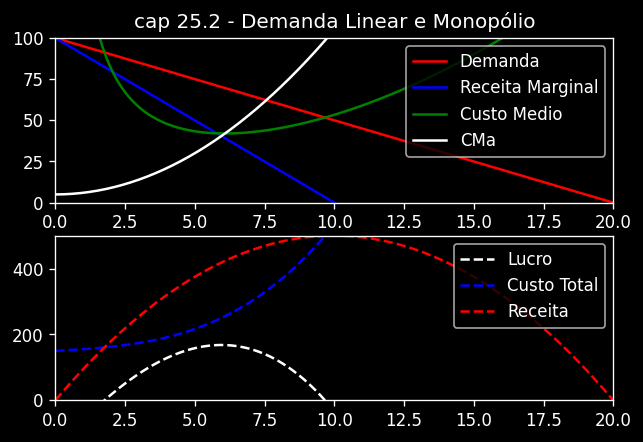
\includegraphics[scale=0.8]{cap25_2-demanda_linear_e_monopolio.png}
\end{center}

Para poder fazer essa simulação, eu tive de definir uma função custo e, consequentemente, uma função custo marginal\footnote{Eu tentei pensar numa função que apresentasse um comportamento parecido com a imagem que vemos no livro.}. Conseguimos ver que a curva de lucro tem um ponto de máximo exatamente onde a curva da receita marginal encontra o custo marginal. Qualquer ponto diferente desse levaria a um nível de lucro menor.
\\
\\
Além disso, também é relevante o fato da curva de custo médio estar abaixo da curva de demanda\footnote{Tente justificar isso matematicamente e, depois, tente criar uma situação onde isso acontece.}. Se o ponto de produção cuja receita marginal é igual ao custo marginal tiver um custo médio superior a demanda, a empresa receberá menos do que os custo de produção.\footnote{Veremos isso daqui a pouco no ponto 25.6.}.

\section{Estabelecimento de Preços com Markup}

Já conseguimos aprimorar nosso modelo de escolha da firma para o caso do monopolista. Agora que tornamos a receita marginal endógena, podemos ver as condições de maximização do lucro quando a firma tem poder de definir o preço ou a quantidade do mercado (mas não os dois ao mesmo tempo).
\\
\\
Podemos compreender essa última equação como uma política de preço do monopolista. Para isso, só precisamos isolar o termo $p(y)$ via rearranjo da última equação, o que após feito nos dá a seguinte relação

$$ p(y) = \frac{CMa(y)}{1 - 1/|\epsilon(y)|} $$
\\
Essa equação nos diz que o preço praticado no mercado cujo monopolista atua sempre\footnote{Sempre que ele agir de acordo com os pressupostos do nosso modelo de escolha.} se comportará como uma função de \textit{markup} do seu custo marginal. Podemos simplificar a visualização disso do seguinte modo

$$ p(y) = \phi \times CMa(y) $$
onde $\phi = \frac{1}{1 - 1/|\epsilon(y)|}$
\\
\\
Como sabemos, o monopolista sempre operará nos pontos cuja demanda é elástica\footnote{Ele até pode operar no ponto onde $\epsilon = 1$, já vimos que nesse caso, o resultado seria o mesmo do caso na competição perfeita.}, isso nos dará um $\epsilon(y) > 1$. Isso nos diz que o divisor $(1 - 1/|\epsilon|) <  1$, o que por sua vez, nos diz que $\phi > 1$.
\\
\\
Agora vamos dar uma olhada em um caso muito interessante: quando a curva de demanda possui a mesma elasticidade em todos os seus pontos.

\subsection{Demanda com Elasticidade Constante e Monopólio}

Para simular o caso da demanda com elasticidade constante, vamos usar o método do markup para encontrar o ponto de oferta do monopolista. Como esperado, teremos uma função de marcação acima da curva de custo marginal.

\begin{center}
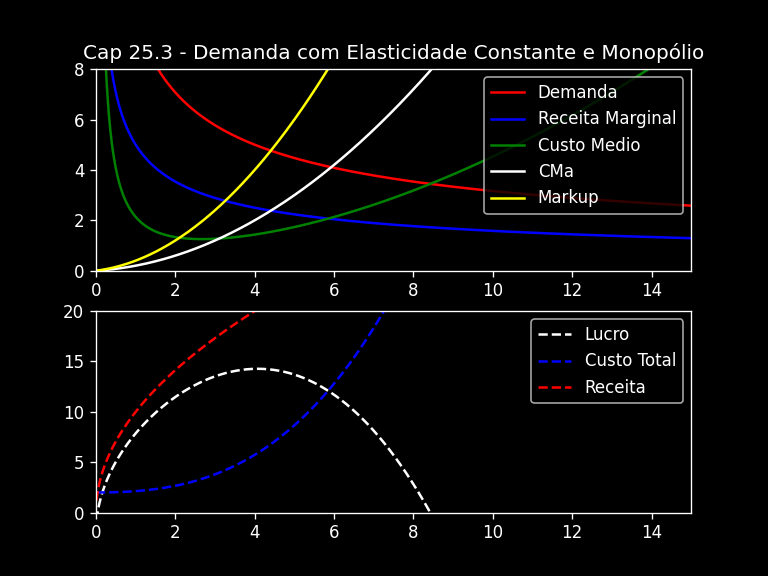
\includegraphics[scale=0.8]{cap25_3-demanda_ces_e_monopolio.png}
\end{center}

\textbf{Simulação:} \href{https://colab.research.google.com/drive/1MRJb9DZ7n_Hz2Kp9ng8K7pOcb1DTy_u5?usp=sharing}{Clique aqui} para ter acesso a essa simulação.
\\
\\
\textbf{Comentário:} Leia o exemplo sobre o impacto dos impostos sobre o monopolista na página 634. Com os conceitos vistos até agora, não deve ser difícil compreende-lo. Você pode acessar a simulação e modificar o custo variável para ver se o resultado é igual ao que você esperava.

\section{A Ineficiência do Monopólio}

Já conseguimos ver que, quando uma empresa opera como um monopólio, o preço de mercado será definido sempre acima do seu custo marginal. No mercado de competição perfeita, esse preço seria exatamente igual ao custo marginal. Isso implica na redução de algum excedente dos consumidores, mas em um incremento no excedente do produtor.
\\
\\
Como já sabemos, um arranjo é eficiente no sentido de Pareto se, e somente se, é possível realizar alguma troca de modo a se ter um aumento no excedente de uma das partes sem a redução do excedente de outra parte. Agora vamos investigar se o equilíbrio no mercado monopolista é eficiente. Considere a imagem abaixo.

\begin{center}
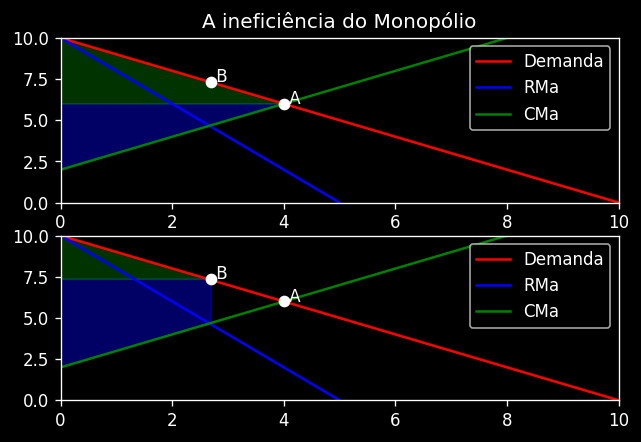
\includegraphics[scale=0.8]{cap25_4-inef_monopolio.png}
\end{center}

No que tange ao equilíbrio no mercado com monopólio. O equilíbrio acontecerá no ponto $B$. A área do retângulo verde acima do retângulo azul é o quanto do excedente do consumidor o monopolista consegue capturar devido o seu poder de mercado. A retângulo azul é precisamente o cenário de equilíbrio no mercado competetivo.
\\
\\
Para investigarmos se há uma ineficiência no sentido de Pareto no ponto $B$, façamos a seguinte pergunta: É possível adicionar uma unidade de produto no mercado, onde o custo marginal pela produção desse bem seja inferior ao preço do mesmo? A resposta é claramente sim!
\\
\\
No nível $B$, a curva de preço (medida pela demanda inversa) ainda é superior à curva de custo marginal (aquela reta verde). Desse modo, se o monopolista produzisse mais uma unidade, ele receberia mais do que o custo marginal dessa unidade e os consumidores cujo preço de reserva é igual ao novo nível de preço passariam a consumir o produto. O excedente desse novo consumidor é igual a $0$, contudo, todos os que já consumiam o produto passaram a pagar menos do que antes o que aumentará os seus respectivos excedentes.

\section{O Ônus do Monopólio}

\begin{center}
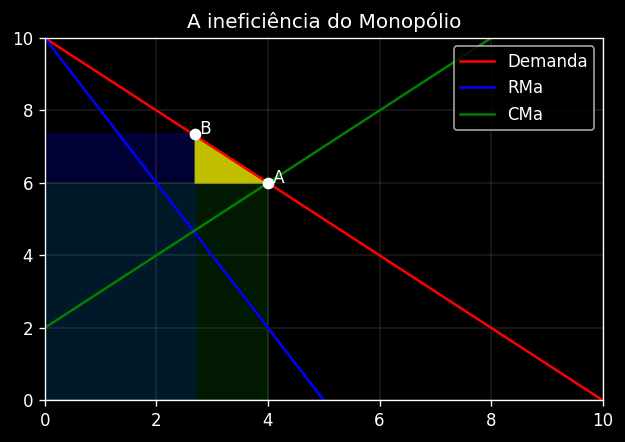
\includegraphics[scale=0.8]{cap25_5-onus_monopolio.png}
\end{center}


\section{Monopólio Natural}
\section{O Que Causa os Monopólios?}

%%%%%%%%%%%%%%%%%%%%%%%% CHAPTER %%%%%%%%%%%%%%%%%%%%%%%%
\chapter{O Comportamento do Monipolista}

%%%%%%%%%%%%%%%%%%%%%%%% CHAPTER %%%%%%%%%%%%%%%%%%%%%%%%
\chapter{O Mercado de Fatores}

%%%%%%%%%%%%%%%%%%%%%%%% CHAPTER %%%%%%%%%%%%%%%%%%%%%%%%
\chapter{O Oligopólio}

%%%%%%%%%%%%%%%%%%%%%%%% CHAPTER %%%%%%%%%%%%%%%%%%%%%%%%
\chapter{A Teoria dos Jogos}

%%%%%%%%%%%%%%%%%%%%%%%% CHAPTER %%%%%%%%%%%%%%%%%%%%%%%%
\chapter{Aplicações da Teoria dos Jogos}

%%%%%%%%%%%%%%%%%%%%%%%% PART %%%%%%%%%%%%%%%%%%%%%%%%
\part{Tópicos Avançados}

%%%%%%%%%%%%%%%%%%%%%%%% CHAPTER %%%%%%%%%%%%%%%%%%%%%%%%
\chapter{Economia Comportamental}

%%%%%%%%%%%%%%%%%%%%%%%% CHAPTER %%%%%%%%%%%%%%%%%%%%%%%%
\chapter{Trocas}

%%%%%%%%%%%%%%%%%%%%%%%% CHAPTER %%%%%%%%%%%%%%%%%%%%%%%%
\chapter{Produção}

%%%%%%%%%%%%%%%%%%%%%%%% CHAPTER %%%%%%%%%%%%%%%%%%%%%%%%
\chapter{O Bem-Estar}

%%%%%%%%%%%%%%%%%%%%%%%% CHAPTER %%%%%%%%%%%%%%%%%%%%%%%%
\chapter{Externalidades}

%%%%%%%%%%%%%%%%%%%%%%%% CHAPTER %%%%%%%%%%%%%%%%%%%%%%%%
\chapter{Tecnologia da Informação}

%%%%%%%%%%%%%%%%%%%%%%%% CHAPTER %%%%%%%%%%%%%%%%%%%%%%%%
\chapter{Bens Públicos}

%%%%%%%%%%%%%%%%%%%%%%%% CHAPTER %%%%%%%%%%%%%%%%%%%%%%%%
\chapter{Informação Assimétrica}

\end{document}
